\documentclass[11pt,a4paper]{article}
\usepackage[utf8]{inputenc}
\usepackage[T1]{fontenc}
\usepackage[portuguese]{babel}
\usepackage{lmodern}
\usepackage[a4paper,top=2.5cm,bottom=2.8cm,left=2.6cm,right=2.6cm]{geometry}
\usepackage{graphicx}
\usepackage{xcolor}
\usepackage{array}
\usepackage{longtable}
\usepackage{enumitem}
\usepackage{titlesec}
\usepackage{fancyhdr}
\usepackage{amssymb}
\usepackage[hidelinks]{hyperref}

\definecolor{ucs}{RGB}{158,27,58}
\DeclareUnicodeCharacter{2248}{\ensuremath{\approx}}
\DeclareUnicodeCharacter{2212}{\ensuremath{-}}
\DeclareUnicodeCharacter{2192}{\ensuremath{\rightarrow}}
\DeclareUnicodeCharacter{00D7}{\ensuremath{\times}}
\DeclareUnicodeCharacter{2264}{\ensuremath{\leq}}
\DeclareUnicodeCharacter{2265}{\ensuremath{\geq}}
\DeclareUnicodeCharacter{03A9}{\ensuremath{\Omega}}
\DeclareUnicodeCharacter{2610}{\ensuremath{\square}}
\DeclareUnicodeCharacter{2612}{\ensuremath{\boxtimes}}

\newcommand{\vazio}{$\square$}
\newcommand{\marcado}{$\boxtimes$}
\newcommand{\parcial}{\textit{\small Parte da entrega parcial de hoje (22h30).}\par\medskip}
\newcommand{\cod}[1]{\texttt{#1}}

\titleformat{\section}{\LARGE\normalfont}{\thesection.}{0.4em}{}
\titleformat{\subsection}{\Large\bfseries}{\thesubsection}{0.4em}{}
\titleformat{name=\section,numberless}{\LARGE\normalfont}{}{0em}{}
\titlespacing*{\section}{0pt}{2.2ex}{1.4ex}

\setlength{\parindent}{0pt}
\setlength{\parskip}{0.5em}
\renewcommand{\arraystretch}{1.15}

\pagestyle{fancy}
\fancyhf{}
\renewcommand{\headrulewidth}{0pt}
\renewcommand{\footrulewidth}{0.4pt}
\fancyfoot[L]{\color{gray}\small Prof. Edson Vaz Lopes}
\fancyfoot[C]{\color{gray}\small\thepage}
\fancyfoot[R]{
\includegraphics[height=0.45cm]{logo.png}}
\fancypagestyle{plain}{}

\begin{document}
\sloppy
\thispagestyle{fancy}

\begin{center}

\includegraphics[height=3.2cm]{logo.png}\par\medskip
{\LARGE\bfseries CP12 --- Proposta de upgrade do projeto N1}\par\smallskip
{\small Internet das Coisas | Aula 12 --- Hardware, firmware-base e contratos}\par
{\small Prof. Edson Vaz Lopes}\par\medskip
{\color{ucs}\rule{\linewidth}{0.6pt}}
\end{center}

\bigskip
\section*{Identificação}

\begin{tabular}{|p{0.45\linewidth}|p{0.45\linewidth}|}
\hline
\textbf{Equipe (nº e nome):} & \textbf{Projeto (N1 $\rightarrow$ N3):} \\ \hline
Equipe HorangoTango & Garagem inteligente: monitoramento de vagas $\rightarrow$ produto \textbf{HorangoTango Park} \\ \hline
\textbf{Integrantes presentes:} & \textbf{Data / Versão:} \\ \hline
Gustavo Vinicius Taques, Luis Fernando Pereira, João Pedro Angelico, Vynicyus Candido & 27/10/2026 -- v1 \\ \hline
\end{tabular}

\section*{Orientações}

Este checkpoint é a \textbf{proposta de upgrade} do projeto que a equipe defendeu na N1 para
o produto da N3: cada seção confere o plano da equipe contra o piso \textbf{R1--R18} definido em
\cod{requisitos\_projeto\_N3.pdf} (documento à parte, \textbf{leitura obrigatória} antes de preencher
este checkpoint).

Da Aula 12 até a N2 (03/11), a Unidade 2 é \textbf{100\% desenho}: não há bancada, não há
circuito montado, não há firmware rodando no ESP32. O que se produz é documentação,
cronograma, fluxogramas, diagrama de blocos e repositório GitHub organizado. A \textbf{Unidade
3} (10/11, 17/11, 24/11) é que \textbf{põe em prática} o que foi desenhado aqui, até a defesa do
produto funcionando na N3 (01/12). Código mostrado neste checkpoint é \textbf{aproximado}:
pode e deve mudar quando for implementado de fato no ESP32.

\textbf{Entrega em duas etapas, hoje -- duas coisas em cada uma: o PDF no Teams e o
repositório no GitHub.}

\begin{itemize}
\item \textbf{Até 22h30 de hoje (20/10):}
  \begin{itemize}[label=--]
  \item PDF com as seções 1 a 4 preenchidas -- ponto de partida, upgrade por camada,
    prova de que a equipe leu o piso R1--R18 e já mapeou cada requisito para o próprio
    projeto, e a arquitetura-alvo esboçada (diagrama de blocos, fluxo do dado e fluxo
    do comando). Nenhuma dessas quatro seções depende de teoria técnica nova --
    usam o que já foi visto na Aula 11 e a leitura autônoma do piso.
  \item Repositório GitHub criado (se ainda não existir) ou atualizado, com um \cod{README.md}
    simples: nome do projeto, problema e usuário, uma frase sobre o estado atual
    (herdado da N1) e para onde o upgrade está indo. Não precisa de instruções de
    instalação ainda -- isso só é exigido no fim (R11, válido para a N3).
  \end{itemize}
\item \textbf{Até o final da Aula 13 (27/10/2026, 22h30):} PDF completo, com as seções 5
  a 9 (hardware calculado, firmware em fluxograma, contrato congelado v1, tecnologias,
  cronograma/riscos/divisão), e repositório atualizado de novo (seção 9). Essas seções
  dependem da teoria de hardware seguro, firmware-base e contratos, dada na própria
  Aula 13 -- a oficina daquela noite é o tempo de aplicar o conteúdo e fechar o documento.
\end{itemize}

Todos os integrantes devem revisar o documento inteiro antes do envio final: o conteúdo é
objeto da prova individual da N2 (03/11). Este checkpoint é a primeira (e única) entrega do
\textbf{T2 -- desenho e documentação do projeto} (grupo, 40\% da N2); a entrega completa, na Aula
13, já congela o contrato como v1 (não há um CP13 separado). A N2 (03/11) = T2 (40\%) +
P2, prova individual de 6 questões (60\%) -- o conteúdo deste checkpoint é também o que cai
na prova.

A partir de hoje, pensem o projeto como \textbf{produto}, não como exercício acadêmico (ver subseção
\textit{Como apresentar} em \cod{requisitos\_projeto\_N3.pdf}): proposta de valor clara, cuidado
visual e praticidade de uso. Isso não tem campo de pontuação próprio neste checkpoint; é a
lente que vale desde já para a interface e o acabamento do hardware.

% ---------------------------------------------------------------- 1
\section{Ponto de partida: o projeto da N1}
\parcial

\begin{longtable}{|p{0.22\linewidth}|p{0.70\linewidth}|}
\hline
Problema e usuário & Em garagens e estacionamentos, o motorista perde tempo circulando à procura de vaga, e o operador não sabe em tempo real quantas vagas estão livres nem há quanto tempo cada uma está ocupada. \textbf{Usuários:} (1) o \textbf{motorista}, que quer saber antes de entrar onde há vaga e ser guiado até ela; (2) o \textbf{operador/administrador} do estacionamento, que monitora a ocupação, configura o sistema e reserva vagas. \\ \hline
O que funcionou na N1 & Sensor ultrassônico HC-SR04 por vaga com histerese (25/35 cm), confirmação por 3 leituras e detecção de falha do sensor (\cod{erro} após 5 leituras inválidas); ESP32 publicando o estado da vaga em MQTT com \textit{retained}; Last Will (\cod{online}/\cod{offline}) por nó; ESP32 atuador com LEDs verde/vermelho assinando o broker (sensor e atuador sem ligação direta); app web de vagas livres via MQTT/WebSocket; broker Mosquitto local documentado; credenciais Wi-Fi fora do código (\cod{secrets.h} no \cod{.gitignore}). \\ \hline
Limitações conhecidas & Sem backend, sem banco e sem histórico; a interface fala direto com o broker; payload em texto puro (\cod{livre}/\cod{ocupada}), sem \cod{deviceId}, timestamp nem unidade; nenhum comando do usuário para o dispositivo (só leitura); broker sem autenticação (\cod{allow\_anonymous true}); limiares fixos no código (não configuráveis remotamente); os LEDs dependiam do broker, então sem rede a vaga ficava sem indicação; o sistema não sabe \textbf{qual} carro está na vaga. \\ \hline
Proposta de valor (por que alguém usaria/compraria este produto) & O motorista abre o app no celular, vê na hora quais vagas estão livres e, na garagem, é guiado pelos LEDs: verde = livre, vermelho = ocupada, azul = reservada. Clientes cadastrados (carro com tag RFID) são identificados ao estacionar e podem ter vaga reservada. O operador ganha ocupação em tempo real, histórico de uso (taxa de ocupação, tempo médio de permanência), alerta no celular quando um sensor falha e reservas com confirmação do hardware --- sem precisar de alguém circulando para conferir as vagas. \\ \hline
\end{longtable}

\textbf{Pedido de troca de projeto:} \vazio\ Sim \qquad \marcado\ Não

Se sim, justificar por que o projeto da N1 não comporta o upgrade e qual problema/usuário
a equipe propõe no lugar. Só é válido com aprovação do professor.

\textit{Histórico da N1:} a proposta inicial, de 26/08 (\cod{docs/IOT\_24\_08.pdf}), era uma balança
de encomendas com sensor de peso. Em 14/09 a equipe a substituiu pela garagem inteligente, por causa
dos recursos de hardware disponíveis e do caminho de crescimento até a N3 com esse hardware. A garagem
é o projeto que funcionou e foi apresentado na N1. Decisão registrada em
\cod{docs/adr/0002-troca-sensor-de-peso-por-garagem.md}.

% ---------------------------------------------------------------- 2
\section{Upgrade por camada}
\parcial

Para cada camada, descrever o estado na N1 e o que muda na N3.

\begin{longtable}{|p{0.17\linewidth}|p{0.33\linewidth}|p{0.40\linewidth}|}
\hline
\textbf{Camada} & \textbf{Como era na N1} & \textbf{Como será na N3} \\ \hline \endhead
Hardware & 2 ESP32 (sensor e atuador), HC-SR04 por vaga, LEDs verde/vermelho por vaga. & 1 ESP32 DevKit (WROOM-32) operando 2 vagas: por vaga, 1 HC-SR04 (presença do carro), 1 leitor RFID RC522 (identificação do carro com tag) e 1 LED RGB (verde/vermelho/azul). Divisor de tensão no Echo, alimentação USB 5 V dimensionada, maquete com acabamento. \\ \hline
Firmware & Dois sketches; leitura com histerese e confirmação; publicação só na mudança; reconexão MQTT; LED só via broker. & Firmware único e não bloqueante: ultrassônico (1 s), RFID (100 ms), LED com \textbf{regra local} (funciona sem rede), estados \textit{automático / reservado (manual) / seguro}, execução de comandos com confirmação, configuração persistente em NVS (limiares e tempo de reserva), \cod{deviceId} pelo MAC, horário por NTP (ou ``hora não sincronizada''), logs no Serial, OTA. \\ \hline
Comunicação (MQTT) & Tópicos \cod{garagem/vaga/N} e \cod{garagem/no/<id>/status}, payload texto, sem contrato escrito. & Contrato versionado (\cod{CONTRATOS.md}, v0 $\rightarrow$ v1 congelado em 27/10): tópicos de telemetria, estado, evento RFID, comando, confirmação e status com Last Will; payload JSON com \cod{v}, \cod{deviceId}, \cod{ts} e unidades; QoS e \textit{retain} justificados por tópico. \\ \hline
Backend & (não existia) & Serviço FastAPI que assina os tópicos do dispositivo, valida cada mensagem contra o contrato (descarta e registra as inválidas), grava no PostgreSQL, executa as regras remotas, envia notificações e expõe a API REST autenticada usada pela interface. É o \textbf{único} que publica comandos. \\ \hline
Banco de dados & (não existia) & PostgreSQL com histórico de medições e de estados das vagas, leituras RFID, registro de comandos (commandId, origem, ação, envio, resultado, confirmação), alertas e usuários. Esquema versionado (migrações). \\ \hline
Interface & App web único que assinava o broker direto e mostrava vagas livres. & (1) \textbf{Painel do operador} (web, com login): estado atual das vagas, histórico e gráficos, online/offline e último contato do dispositivo, alertas ativos, tags lidas, envio de reserva e alteração de configuração. (2) \textbf{App do motorista} (web responsivo no celular): vagas livres em tempo real e destaque da vaga do motorista com tag. Ambos falam só com a API do backend. \\ \hline
Decisão/regra & Só local: histerese e confirmação no ESP32. & \textbf{Local (firmware):} histerese, confirmação, estado seguro em falha de sensor e LED seguindo o sensor mesmo sem rede. \textbf{Remota (backend):} reserva expira se o carro não chegar no tempo configurado $\rightarrow$ backend envia comando \cod{cancelar\_reserva}; sensor em \cod{erro} ou dispositivo \cod{offline} por mais de 1 min $\rightarrow$ alerta e notificação no Telegram. \\ \hline
\end{longtable}

% ---------------------------------------------------------------- 3
\section{Conferência contra o piso R1--R18}
\parcial

Para cada requisito do piso (ver \cod{requisitos\_projeto\_N3.pdf}), uma frase sobre como o
projeto pretende atendê-lo. Quem ainda não sabe, escreve a pendência -- não deixar em
branco. Vários requisitos de R12 a R18 já foram implementados por algumas equipes na N1:
nesse caso, descrever o que já existe e o que falta evoluir.

\begin{longtable}{|p{0.15\linewidth}|p{0.77\linewidth}|}
\hline
\textbf{Req.} & \textbf{Como o projeto vai atender} \\ \hline \endhead
R1 Hardware & ESP32 com \textbf{duas entradas de tipos diferentes} por vaga (HC-SR04 = distância/presença; RC522 = identificação RFID) em \textbf{dois pontos de medição} (vagas 1 e 2) e \textbf{atuador real}: LED RGB por vaga (verde/vermelho/azul) com resistor. Mapa de pinos (\cod{docs/mapa-de-pinos.md}), BOM e esquema elétrico no repositório; maquete com fiação fixa. \\ \hline
R2 Firmware & Laço com \cod{millis()} sem \cod{delay()} longo (ultrassônico a cada 1 s, RFID a cada 100 ms); leituras validadas (faixa 2--400 cm, eco ausente como sentinela, leitor RC522 verificado a cada 5 s); \textbf{regra local sem rede}: LED segue o estado confirmado do sensor mesmo com Wi-Fi/broker fora; \textbf{estado seguro}: falha de sensor $\rightarrow$ vaga \cod{erro}, LED vermelho piscando (nunca verde sem certeza); reconexão automática ao Wi-Fi e ao broker refazendo as assinaturas; \textbf{configuração persistente} em NVS (limiares e duração da reserva, alteráveis por comando \cod{configurar}); \cod{deviceId} derivado do MAC; timestamp via NTP ou campo \cod{ts\_sincronizado: false}; logs no Serial. \\ \hline
R3 Contrato MQTT & \cod{CONTRATOS.md} com árvore de tópicos (telemetria, estado, rfid, cmd, ack, status/LWT), exemplo JSON por tópico com \cod{v}, \cod{deviceId}, \cod{ts} e unidades, comandos aceitos e faixas, confirmação com \cod{commandId} e resultado, catálogo de erros, QoS/retain justificados. v0 em 20/10; v1 congelado em 27/10 (seção 6). \\ \hline
R4 Backend & FastAPI + cliente MQTT assinando \cod{garagem/v1/\#}; validação com Pydantic contra o contrato (inválidas descartadas e gravadas em \cod{mensagens\_invalidas}); persistência no PostgreSQL; API REST: estado atual, histórico, alertas, envio de comando; único publicador de \cod{cmd}. \\ \hline
R5 Banco de dados & PostgreSQL com tabelas \cod{dispositivos}, \cod{medicoes} (dispositivo, vaga, grandeza, valor, unidade, ts), \cod{estados\_vaga}, \cod{leituras\_rfid}, \cod{comandos} (commandId, origem, ação, enviado\_em, resultado, confirmado\_em, motivo), \cod{alertas}, \cod{usuarios}. Migrações versionadas (Alembic). \\ \hline
R6 Interface & Painel web do operador: distância atual (cm) e estado de cada vaga, histórico (tabela e gráfico), último contato e online/offline do dispositivo, alertas ativos, botão de reserva e formulário de configuração (limiares, tempo de reserva). App do motorista: vagas livres e vaga destacada pela tag. \\ \hline
R7 Ciclo de comando & Comando \cod{reservar} (e \cod{cancelar\_reserva}, \cod{configurar}) com estados distintos gravados no banco e exibidos na interface: \textbf{enviado} (backend publicou) $\rightarrow$ \textbf{recebido} (ESP32 aceitou ou rejeitou, com motivo) $\rightarrow$ \textbf{executado} (LED ficou azul) $\rightarrow$ \textbf{confirmado} (estado \cod{reservada} publicado e refletido na interface). Intertravamento: reservar vaga ocupada ou em erro é rejeitado com \cod{VAGA\_OCUPADA} / \cod{VAGA\_EM\_ERRO}. \\ \hline
R8 Decisão remota & Regra no backend: reserva sem chegada do carro dentro do tempo configurado pelo operador (padrão 15 min, salvo no banco) $\rightarrow$ backend gera \cod{cancelar\_reserva} com o mesmo ciclo do R7 e registra alerta. Segunda regra: vaga em \cod{erro} ou dispositivo \cod{offline} > 1 min $\rightarrow$ alerta (R15). \\ \hline
R9 Segurança básica & Login com usuário/senha (hash bcrypt) e token JWT na interface e nas rotas de comando; só usuário autenticado envia comando. Credenciais de Wi-Fi e broker no ESP32 em \cod{secrets.h} (ignorado pelo Git, já existe desde a N1); banco, broker e app em \cod{.env} com \cod{.env.example} versionado; Mosquitto com usuário/senha (fim do \cod{allow\_anonymous}). \\ \hline
R10 Falhas testadas & Plano com 4+ cenários, cada um com provocação, esperado, observado e evidência (log/vídeo/print): (1) queda do Wi-Fi $\rightarrow$ LED segue sensor local, reconecta e republica; (2) broker indisponível $\rightarrow$ idem, interface mostra offline via LWT; (3) falha de sensor (Echo desconectado) $\rightarrow$ \cod{erro}, estado seguro e alerta; (4) comando inválido/duplicado $\rightarrow$ rejeitado com código, \cod{commandId} repetido não reexecuta. Extra: RC522 desconectado $\rightarrow$ identificação para, vaga segue funcionando. \\ \hline
R11 Entrega executável & README com pré-requisitos, \cod{.env.example}, \cod{docker compose up} para broker/backend/banco, gravação do firmware (Arduino IDE/arduino-cli) e reaproveitamento declarado; release/tag \cod{v1.0} da versão defendida; commits de todos os integrantes. \\ \hline
R12 Orquestração (Docker Compose) & \cod{compose.yaml} com \cod{mosquitto} (config + senhas), \cod{postgres} (volume persistente), \cod{backend} (FastAPI, também serve painel e app). Variáveis sensíveis via \cod{.env}. Um único \cod{docker compose up -d}. \\ \hline
R13 Múltiplos dispositivos & \textbf{Pendência -- não atendido no desenho atual.} A equipe decidiu usar \textbf{um único ESP32} para as duas vagas, o que dá um só \cod{deviceId}. O backend, o contrato (\cod{deviceId} em todo tópico) e a interface já são desenhados para N dispositivos. Alternativa avaliada para atender: um ESP32 por vaga com o mesmo firmware (a placa reserva já está na BOM). Decisão pendente com o professor. \\ \hline
R14 Painel analítico & Gráficos na própria interface (Chart.js) com dados reais do banco: taxa de ocupação por hora do dia, tempo médio de permanência por vaga, uptime do dispositivo e tempo em \cod{erro}. \\ \hline
R15 Notificação externa & Bot do Telegram acionado pelo backend quando um sensor entra em \cod{erro}, o dispositivo fica \cod{offline} > 1 min ou uma reserva expira. \\ \hline
R16 Segurança avançada (TLS/perfis) & Perfis com permissões diferentes na API e na interface: \textbf{operador} (visualiza estado, histórico e alertas) e \textbf{administrador} (reserva vagas, altera configuração, gerencia tags). Verificado no backend em cada rota. TLS no MQTT avaliado como extra; se não implementado, justificativa registrada (rede local isolada). \\ \hline
R17 OTA & ArduinoOTA (ou \cod{HTTPUpdate} baixando o binário do backend), com senha de OTA em \cod{secrets.h}. Demonstração: gravar nova versão pela rede e conferir a versão publicada no status. \\ \hline
R18 Testes e CI & \cod{pytest} no backend: validação de contrato (payloads válidos/inválidos), ciclo de comando e regra de expiração da reserva; GitHub Actions rodando os testes (e compilando o firmware com \cod{arduino-cli}) a cada push/PR. \\ \hline
\end{longtable}

% ---------------------------------------------------------------- 4
\section{Arquitetura-alvo}
\parcial

Desenhar (aqui ou em anexo) o diagrama de blocos e os dois fluxos da N3.

\begin{center}
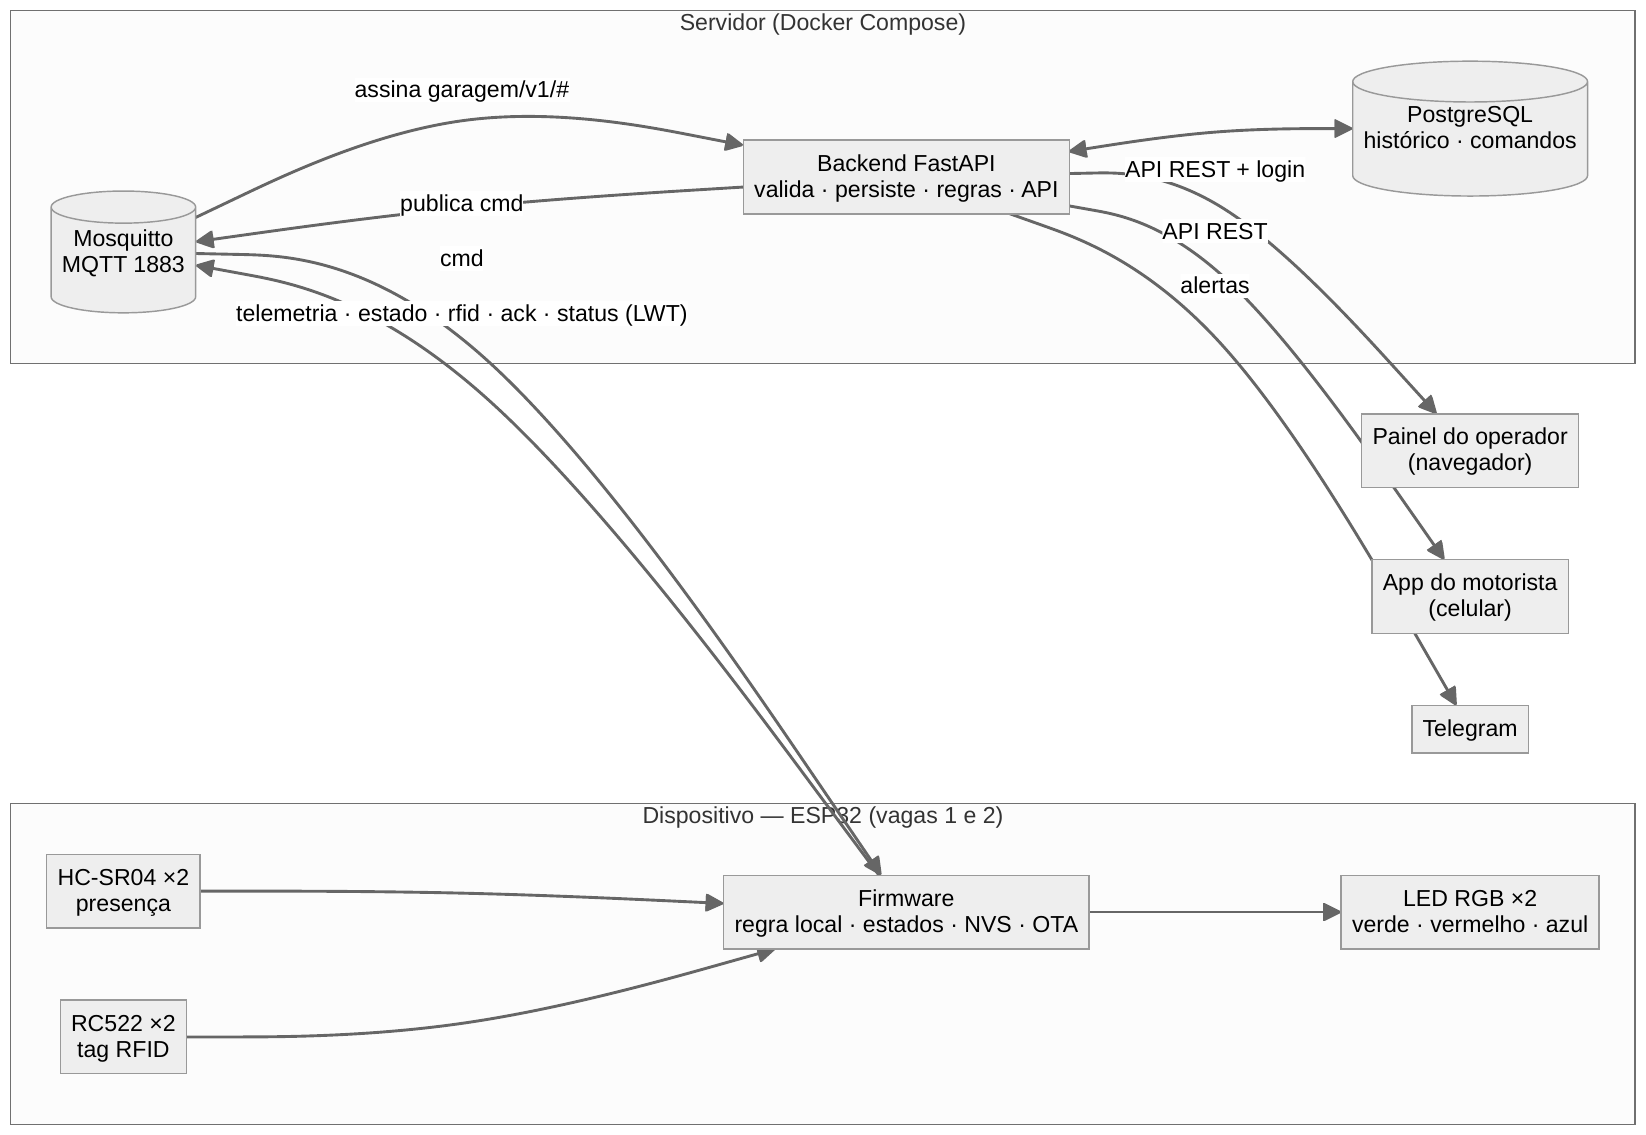
\includegraphics[width=0.95\linewidth]{diag1.png}
\end{center}

\textbf{Fluxo do dado} (sensor $\rightarrow$ firmware $\rightarrow$ MQTT $\rightarrow$ backend $\rightarrow$ banco $\rightarrow$ interface):

\begin{center}
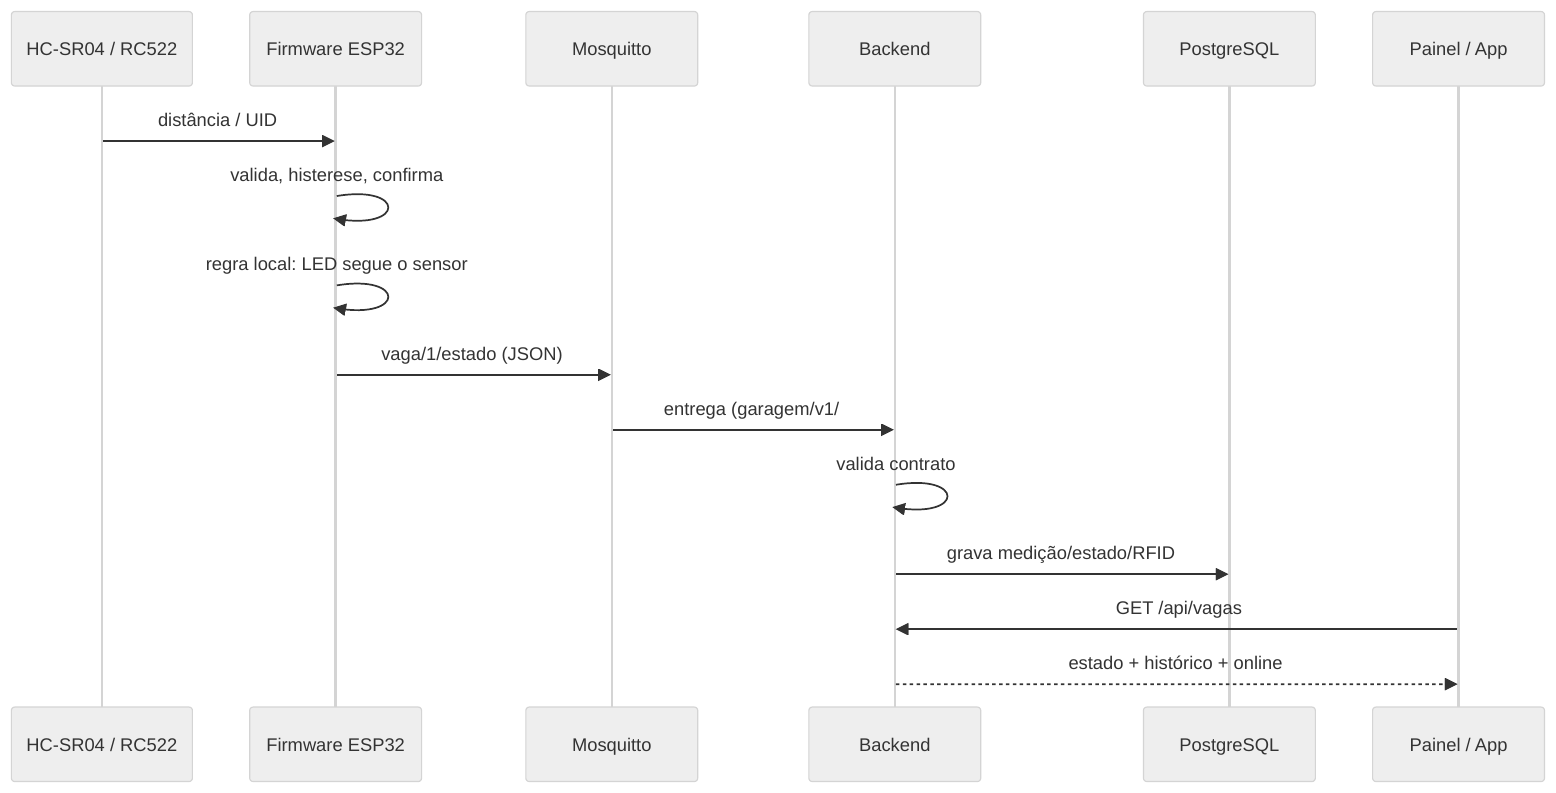
\includegraphics[width=0.95\linewidth]{diag2.png}
\end{center}

\textbf{Fluxo do comando} (interface $\rightarrow$ backend $\rightarrow$ MQTT $\rightarrow$ firmware $\rightarrow$ atuador $\rightarrow$ confirmação):

\begin{center}
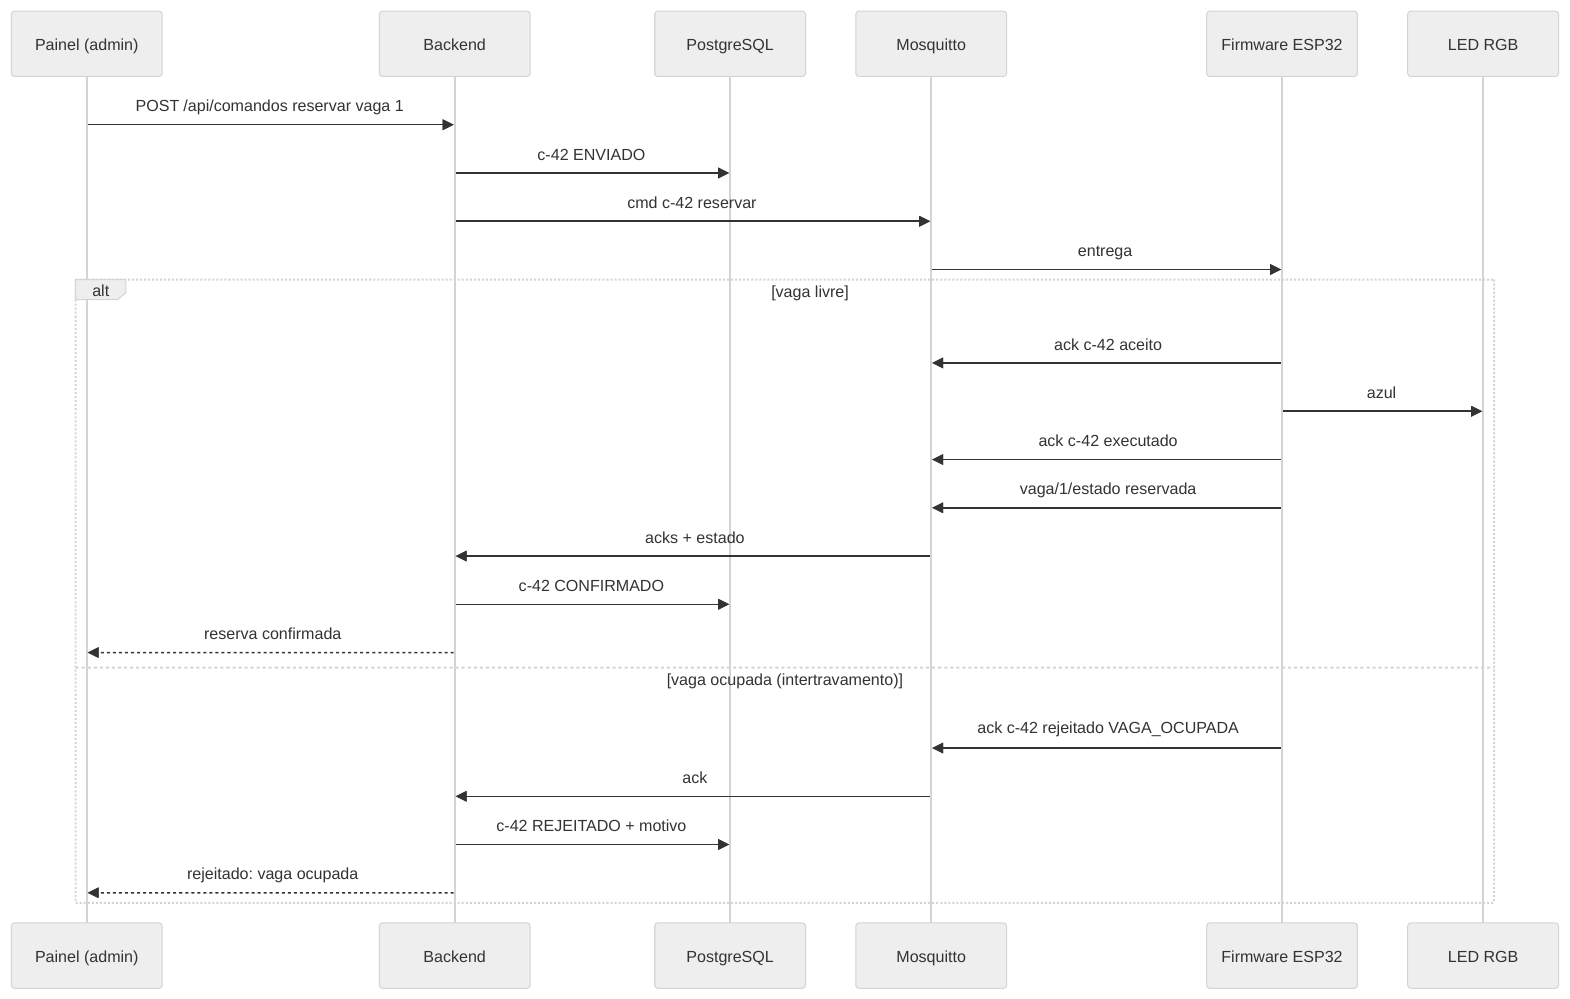
\includegraphics[width=0.95\linewidth]{diag3.png}
\end{center}

% ---------------------------------------------------------------- 5
\section{Hardware: desenho e dimensionamento}
\subsection*{5.1 Verificação elétrica (calculada)}

Sem bancada nesta etapa: os valores abaixo são \textbf{calculados a partir do datasheet} dos
componentes escolhidos, não medidos. Anexar o esquema elétrico desenhado (à mão, Fritzing,
KiCad ou equivalente) -- não é preciso o circuito físico montado.

\begin{longtable}{|p{0.28\linewidth}|p{0.34\linewidth}|p{0.28\linewidth}|}
\hline
\textbf{Verificação} & \textbf{Valor calculado/esperado} & \textbf{Como será garantido} \\ \hline \endhead
Tensão no pino 3V3 e 5V/VIN usados & VIN = 5,0 V (USB); 3V3 = 3,3 V do regulador AMS1117 da placa (até 1 A). Carga no 3V3 ≈ ESP32 (pico ≈240 mA com Wi-Fi) + 2× RC522 (≈26 mA cada) ≈ 300 mA. & RC522 só no 3V3; HC-SR04 no VIN; fonte USB 5 V / 1 A (consumo total estimado ≈350 mA de pico). \\ \hline
Corrente estimada do(s) atuador(es) & LED vermelho: (3,3 − 2,0) / 220 Ω ≈ 5,9 mA. Verde/azul: (3,3 − 3,0) / 68 Ω ≈ 4,4 mA. Um canal aceso por vaga → ≤ 6 mA por GPIO, ≤ 12 mA no total. & Resistor em série em cada canal; abaixo do limite recomendado do GPIO (≈20 mA) e do absoluto (40 mA). \\ \hline
GND comum entre todas as fontes previstas & Uma única fonte (USB). & Trilha de GND única na protoboard ligando ESP32, HC-SR04, RC522 e LEDs. \\ \hline
Maior tensão que chegará a um GPIO (qual sensor?) & HC-SR04 Echo = 5 V → divisor 1 kΩ / 2 kΩ: 5 × 2/3 = \textbf{3,33 V} nos GPIO 34/35. RC522 opera em 3,3 V. & Divisor em cada Echo (ou HC-SR04P de 3,3 V, sem divisor). Conferir com multímetro na montagem. \\ \hline
Proteção planejada para carga indutiva (se houver) & Não há carga indutiva (sem relé, motor ou bomba). & --- \\ \hline
Estado seguro definido para o atuador no boot & LEDs \textbf{apagados} desde o \cod{setup()} (pinos em \cod{OUTPUT LOW}) até o primeiro estado confirmado do sensor; nenhum LED em pino de strapping. & Pinos dos LEDs (32, 33, 27, 13, 16, 17) sem função de boot; firmware inicializa antes de qualquer conexão. \\ \hline
\end{longtable}

Conferir no desenho:

\begin{itemize}[label={}, leftmargin=1.5em]
\item \marcado\ Nenhuma carga (motor, bomba, relé, cooler, fita de LED) alimentada diretamente por GPIO no esquema. \textit{(Só LEDs indicadores com resistor, ≤ 6 mA.)}
\item \marcado\ Carga indutiva com diodo de roda livre previsto (ou módulo que já o inclua --- indicar qual). \textit{(Não se aplica: sem carga indutiva.)}
\item \marcado\ Nenhum sinal de 5 V ligado direto a um GPIO no desenho (divisor ou conversor de nível quando necessário). \textit{(Divisor no Echo do HC-SR04.)}
\item \marcado\ Nenhum uso de GPIO 6--11; nenhum atuador em pino de \textit{strapping} (0, 2, 5, 12, 15) sem justificativa. \textit{(GPIO 5 usado só como SS do RC522 --- SS padrão do SPI, com pull-up interno que mantém o leitor desselecionado e o nível exigido no boot.)}
\item \marcado\ Sensores analógicos planejados no ADC1 (GPIO 32--39), já que o ADC2 não lê com Wi-Fi ativo. \textit{(Não se aplica: HC-SR04 e RC522 são digitais.)}
\end{itemize}

\textbf{Esquema elétrico:} pendente (Fritzing), a versionar em \cod{docs/}.

\subsection*{5.2 BOM e mapa de pinos}

\begin{longtable}{|p{0.25\linewidth}|p{0.67\linewidth}|}
\hline
BOM -- o que já tem & 1× ESP32 DevKit 30 pinos (ESP32-WROOM-32, USB-C, CP2102). \textit{(Equipe completar.)} \\ \hline
BOM -- o que falta comprar/providenciar & 1× ESP32 reserva; 2× HC-SR04; 2× RC522 + 4--6 tags 13,56 MHz (MIFARE 1K); 2× LED RGB catodo comum; resistores 2× 220 Ω, 4× 68--100 Ω, 2× 1 kΩ, 2× 2 kΩ; 2 protoboards 830 furos; jumpers; cabo USB-C de dados; fonte USB 5 V / 1 A; roteador Wi-Fi 2,4 GHz; servidor (PC/notebook/Raspberry Pi); maquete (base, suportes, carrinhos). \\ \hline
Caminho do mapa de pinos no repositório & \cod{docs/mapa-de-pinos.md} \\ \hline
\end{longtable}

\subsection*{5.3 Fluxograma do firmware}

Desenhar os estados do firmware (pelo menos automático, manual e seguro), indicando em
cada transição o evento que a provoca, o timeout do modo manual e a condição de inter-
travamento. É um fluxograma de design: a implementação real no ESP32 pode ajustar
detalhes.

\begin{center}
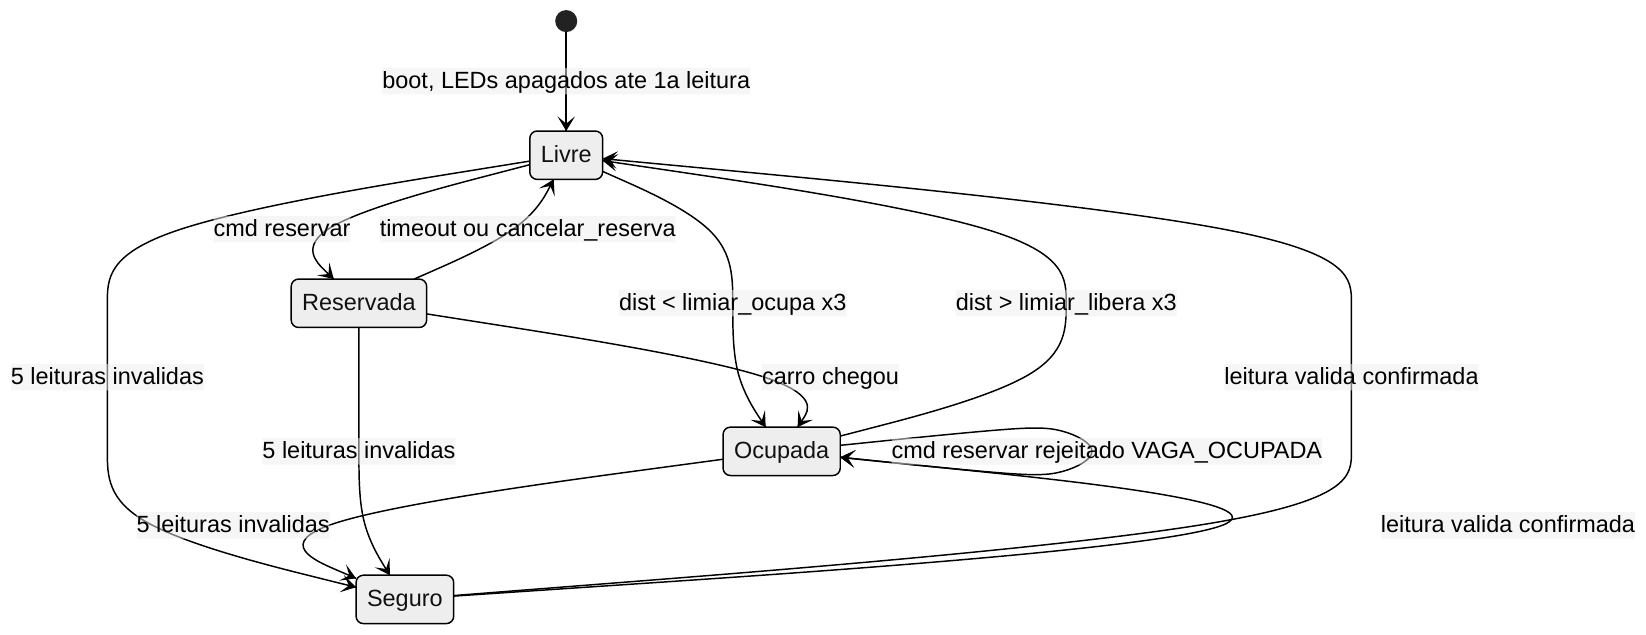
\includegraphics[width=0.85\linewidth]{diag4.png}
\end{center}

\begin{longtable}{|p{0.15\linewidth}|p{0.28\linewidth}|p{0.17\linewidth}|p{0.30\linewidth}|}
\hline
\textbf{Estado} & \textbf{Modo} & \textbf{LED} & \textbf{Saída} \\ \hline
Livre / Ocupada & \textbf{Automático} (regra local, funciona sem rede) & verde / vermelho & sensor confirma mudança (3 leituras) \\ \hline
Reservada & \textbf{Manual} (por comando) & azul & \textbf{timeout} da reserva (\cod{duracao\_min}, padrão 15 min, em NVS --- conta mesmo sem rede), \cod{cancelar\_reserva} ou carro detectado \\ \hline
Seguro & \textbf{Seguro} (falha de sensor, publica \cod{erro}) & vermelho piscando, nunca verde & leitura válida confirmada \\ \hline
\end{longtable}

\textbf{Intertravamento:} \cod{reservar} só é aceito com a vaga \textbf{Livre}; em Ocupada $\rightarrow$ \cod{VAGA\_OCUPADA}, em Seguro $\rightarrow$ \cod{VAGA\_EM\_ERRO}.

Paralelo aos estados, o laço principal (sem \cod{delay()} longo): verifica Wi-Fi/MQTT e reconecta refazendo a assinatura de \cod{cmd} $\rightarrow$ lê ultrassônico (1 s) $\rightarrow$ lê RFID (100 ms) $\rightarrow$ atualiza LED $\rightarrow$ publica pendentes $\rightarrow$ processa comandos (aceita/rejeita, executa, confirma) $\rightarrow$ telemetria periódica (10 s). Detalhes em \cod{docs/fluxograma-firmware.md}.

% ---------------------------------------------------------------- 6
\section{Contrato v0}

Na entrega parcial de hoje, ainda não precisa estar congelado. Na entrega completa (final
da Aula 13), já deve estar congelado como v1. Escrever a árvore de tópicos pretendida e um
exemplo de payload.

\textbf{Congelado como v1 em 27/10/2026.} Contrato completo, com exemplo de payload por tópico, comandos, faixas e códigos de erro, em \cod{CONTRATOS.md}.

\begin{longtable}{|p{0.22\linewidth}|p{0.70\linewidth}|}
\hline
Árvore de tópicos & {\small \ttfamily\raggedright
garagem/v1/\{id\}/telemetria \hfill QoS 0, sem retain\newline
garagem/v1/\{id\}/vaga/\{n\}/estado \hfill QoS 1, retain\newline
garagem/v1/\{id\}/rfid \hfill QoS 1, sem retain\newline
garagem/v1/\{id\}/cmd \hfill QoS 1, sem retain\newline
garagem/v1/\{id\}/ack \hfill QoS 1, sem retain\newline
garagem/v1/\{id\}/status (LWT) \hfill QoS 1, retain}
\smallskip
{\small \cod{\{id\}} = \cod{deviceId} (ex.: \cod{esp32-garagem-240ac4000110}). Estado: \cod{livre} / \cod{ocupada} / \cod{reservada} / \cod{erro}. Comandos: \cod{reservar}, \cod{cancelar\_reserva}, \cod{configurar}. Ack: \cod{aceito} / \cod{rejeitado} / \cod{executado} + \cod{commandId}.} \\ \hline
Exemplo de payload (telemetria ou estado) & {\small \ttfamily
// garagem/v1/esp32-garagem-240ac4000110/vaga/1/estado\newline
\{ "v": 1, "deviceId": "esp32-garagem-240ac4000110",\newline
\ \ "ts": "2026-10-27T21:30:05Z", "vaga": 1, "estado": "ocupada",\newline
\ \ "distancia": \{ "valor": 12.4, "unidade": "cm" \} \}\newline\vspace{0.4em}
// garagem/v1/esp32-garagem-240ac4000110/ack\newline
\{ "v": 1, "deviceId": "esp32-garagem-240ac4000110",\newline
\ \ "ts": "2026-10-27T21:31:01Z", "commandId": "c-0042",\newline
\ \ "resultado": "rejeitado", "erro": "VAGA\_OCUPADA" \}} \\ \hline
\end{longtable}

% ---------------------------------------------------------------- 7
\section{Tecnologias pretendidas}

Escolha livre de linguagem, framework, banco e interface (ver seção 4.1 de \cod{requisitos\_projeto\_N3.pdf}):
vedadas plataformas prontas e fechadas em que backend, regras, banco ou interface não
possam ser inspecionados no repositório (ex.: Blynk, Arduino IoT Cloud). Em caso de
dúvida, perguntar antes de escolher.

\begin{longtable}{|p{0.20\linewidth}|p{0.30\linewidth}|p{0.40\linewidth}|}
\hline
\textbf{Camada} & \textbf{Tecnologia escolhida} & \textbf{Justificativa} \\ \hline \endhead
Backend & Python 3.12 + FastAPI + aiomqtt & Sugestão da disciplina; validação de contrato com Pydantic; documentação automática da API (OpenAPI); \cod{pytest} simples para R18. \\ \hline
Banco de dados & PostgreSQL 16 + SQLAlchemy/Alembic & Relacional recomendado; consultável ao vivo (psql); migrações versionadas para R5. \\ \hline
Interface & Web (HTML/CSS/JS) servida pelo backend + Chart.js; app do motorista responsivo (PWA) & Evolui o app da N1 sem build; roda no navegador do celular sem instalação; gráficos do R14 sem ferramenta externa. \\ \hline
Broker MQTT & Eclipse Mosquitto 2 & Já usado na N1; leve, aberto, suporta usuário/senha, ACL, WebSocket e TLS. \\ \hline
Orquestração (Docker Compose) & Docker Compose: \cod{mosquitto}, \cod{postgres}, \cod{backend} & Sobe os três serviços com \cod{docker compose up -d}; segredos em \cod{.env}. \\ \hline
\end{longtable}

% ---------------------------------------------------------------- 8
\section{Cronograma, riscos e divisão de responsabilidades}
\subsection*{8.1 Cronograma até a N3}

\begin{longtable}{|p{0.13\linewidth}|p{0.22\linewidth}|p{0.55\linewidth}|}
\hline
\textbf{Data} & \textbf{Marco} & \textbf{O que a equipe entrega} \\ \hline \endhead
27/10 & CP12 completo (fim da Aula 13) + contrato congelado v1 & PDF completo; \cod{CONTRATOS.md} v1; esquema elétrico; fluxograma do firmware; modelo de dados; esboço das telas; plano de testes dos 4 cenários; repositório atualizado com commit de todos. \\ \hline
03/11 & N2 & T2 (este documento + repositório) e prova individual P2. \\ \hline
10/11 -- 24/11 & Unidade 3 & \textbf{10/11:} hardware montado na maquete, firmware com contrato v1, regra local, NVS (R1--R3); \cod{compose.yaml} com broker + banco + backend esqueleto (R12). \textbf{17/11:} backend validando e persistindo, API, painel com login e ciclo de comando (R4--R7, R9). \textbf{24/11:} regra remota, Telegram, gráficos, perfis, OTA, testes + CI, falhas testadas com evidência (R8, R10, R14--R18). \\ \hline
01/12 & N3 & Release \cod{v1.0} no GitHub; README executável (R11); defesa do produto funcionando. \\ \hline
\end{longtable}

\subsection*{8.2 Riscos}

\begin{longtable}{|p{0.42\linewidth}|p{0.50\linewidth}|}
\hline
\textbf{Risco} & \textbf{Mitigação} \\ \hline \endhead
R13 não atendido com um único ESP32. & Backend e contrato já suportam N dispositivos; decisão pendente com o professor; placa reserva na BOM permite dividir uma vaga por ESP32 sem mudar o firmware. \\ \hline
Atraso na compra de RC522/tags/LED RGB. & RFID é complementar --- o sistema funciona só com ultrassônico; tags podem ser publicadas manualmente (\cod{mosquitto\_pub}) nos testes. \\ \hline
Dois RC522 no mesmo SPI não se entenderem. & SS separados, todos em nível alto antes do \cod{SPI.begin}; verificação periódica com reinicialização; testar cedo (10/11). \\ \hline
Rede da faculdade bloqueia ESP32/celulares (WPA2-Enterprise, isolamento). & Roteador 2,4 GHz próprio para a demonstração. \\ \hline
Calibração do ultrassônico na maquete. & Limiares configuráveis pela interface (NVS) --- ajuste sem regravar. \\ \hline
Escopo grande (R12--R18) para 3 aulas. & Priorizar R1--R11 em 10/11 e 17/11; R12 desde o início (compose); R14--R18 em 24/11; divisão por camada. \\ \hline
ESP32 único é ponto único de falha. & LWT + alerta; estado seguro; regra local sem rede; placa reserva. \\ \hline
\end{longtable}

\subsection*{8.3 Divisão de responsabilidades}

\begin{longtable}{|p{0.32\linewidth}|p{0.60\linewidth}|}
\hline
\textbf{Integrante} & \textbf{Responsabilidade principal até a entrega completa (Aula 13)} \\ \hline \endhead
Gustavo Vinicius Taques & Hardware: esquema elétrico (Fritzing), verificação elétrica, BOM \\ \hline
Luis Fernando Pereira & Firmware: fluxograma de estados, mapa de pinos, contrato v1 (\cod{CONTRATOS.md}) \\ \hline
João Pedro Angelico & Backend e banco: modelo de dados, endpoints da API, regra remota, \cod{compose.yaml} planejado \\ \hline
Vynicyus Candido & Interface: esboço das telas (painel e app do motorista), plano de testes de falha, repositório/README \\ \hline
\end{longtable}

% ---------------------------------------------------------------- 9
\section{Repositório (GitHub) -- 1,0 ponto fixo (25\% do T2)}

O repositório é a segunda entrega de hoje, junto com este PDF (ver Orientações). Precisa
existir com um \cod{README.md} simples -- nome do projeto, problema e usuário, estado atual
(herdado da N1) e para onde o upgrade está indo -- desde às 22h30. Não é o README de
instalação completo: isso só é exigido para a N3 (R11).

\textbf{A partir de 20/10/2026, a completude do repositório tem nota própria e fixa
dentro do T2: 1,0 ponto dos 4,0, avaliado na entrega completa (final da Aula 13).}
O princípio é simples: o PDF é a proposta, o repositório é a prova -- o que está escrito aqui
precisa existir, de fato, versionado no GitHub.

Critério de avaliação:

\begin{itemize}
\item \textbf{Completo (1,0 ponto)} -- todos os itens presentes: repositório \textbf{público} (acessível
  sem convite); \cod{README.md} completo (projeto, problema, usuário, estado atual, direção
  do upgrade); \textbf{diagramas e gráficos} versionados no repositório (arquitetura-alvo, fluxograma do firmware, esquema elétrico -- não apenas texto); conteúdo do repositório
  \textbf{correspondendo exatamente} ao que foi entregue em PDF (mesmo commit, sem
  divergência); \textbf{commit de cada integrante} da equipe.
\item \textbf{Parcial (0,5 ponto)} -- falta um item secundário: por exemplo, só texto sem diagramas
  versionados, ou commits concentrados em 1--2 integrantes.
\item \textbf{Insuficiente (0 ponto)} -- repositório não existe, não é público, ou diverge do PDF
  entregue.
\end{itemize}

\begin{longtable}{|p{0.25\linewidth}|p{0.67\linewidth}|}
\hline
Link do repositório & \url{https://github.com/VynicyusCandido/iotHorangoTango} \\ \hline
Hash do commit entregue & tag \cod{cp12-v1} -- commit que contém este PDF e o \cod{docs/cp12/CP12.tex} que o gerou \\ \hline
\end{longtable}

\begin{longtable}{|p{0.45\linewidth}|p{0.47\linewidth}|}
\hline
\textbf{Integrante} & \textbf{Usuário GitHub (com commit próprio no repositório)} \\ \hline
Gustavo Vinicius Taques & \textit{(pendente: sem commit no repositório)} \\ \hline
Luis Fernando Pereira & Luis-Fernando-Pereira \\ \hline
João Pedro Angelico & joaopedroangelico \\ \hline
Vynicyus Candido & VynicyusCandido \\ \hline
\end{longtable}

\section*{Checklist antes do envio}

\begin{itemize}[label={}, leftmargin=1.5em]
\item \marcado\ Seções 1 a 4 enviadas até 22h30 de hoje (mesmo que o resto ainda esteja em branco).
\item \marcado\ Repositório no GitHub criado/atualizado até 22h30, com \cod{README.md} simples apontando
  para onde o projeto está indo. \textbf{Repositório público} -- o ponto do GitHub (seção 9)
  exige acesso sem convite.
\item \marcado\ Tabela de verificação elétrica preenchida com valores \textbf{calculados}, não medidos -- sem
  bancada nesta etapa.
\item \vazio\ Esquema elétrico desenhado anexado (não é necessário circuito físico montado).
\item \marcado\ Fluxograma do firmware desenhado.
\item \marcado\ Conferência R1--R18 sem linha em branco (pendências declaradas, não omitidas).
\item \marcado\ Cronograma até a N3 preenchido.
\item \marcado\ Tecnologias pretendidas justificadas; nenhuma plataforma fechada da seção 4.1.
\item \vazio\ Repositório com commit de cada integrante listado.
\item \vazio\ Todos os integrantes revisaram o documento completo antes do envio final.
\end{itemize}

\section*{Entrega}

Duas etapas, cada uma com duas coisas -- \textbf{PDF no Teams} e \textbf{repositório no GitHub}:

\begin{enumerate}
\item \textbf{Até 22h30 de hoje (20/10):} PDF com pelo menos as seções 1 e 3 (nome sugerido:
  \cod{CP12\_EQUIPE-X\_PARCIAL.pdf}) e repositório criado/atualizado com \cod{README.md} simples
  (projeto, problema, usuário, estado atual, direção do upgrade).
\item \textbf{Até o final da Aula 13 (27/10/2026, 22h30):} PDF completo, com todas as seções
  (nome sugerido: \cod{CP12\_EQUIPE-X\_PROJETO\_v1.0.pdf}) e repositório atualizado de novo,
  com o contrato já congelado como v1.
\end{enumerate}

\end{document}
